

\section{Benchmark Problems}
\label{sec:benchmarks}

In this section we will test the performance of our designed algorithm (path representation) using some larger benchmark problems. Again we tested the parameter values in table \ref{table:question_3}. We came to the conclusion that the parameter values found in table \ref{table:question_3} are also good parameter values for larger benchmark problems. We executed the tests on the benchmark problem containing 380 cities (\texttt{bcl380.tsp}). It is certainly not that logical that the parameter values that are optimal for small size problems are also the optimal values for larger size problems. Now that we have found good parameter settings for our genetic algorithm, we can use the algorithm to solve some large benchmark problems.
In figure \ref{fig:belgium_tour_4} you can see the results for the Belgium tour benchmark problem. It seems that the GA found a good solution very quickly. 
\newline
\newline
We also did a performance comparison of the original GA (adjacency representation) with the newly designed GA (path representation). For both algorithms their best found set of parameter values are used. In figure \ref{fig:adj_vraag4_off_gen} and \ref{fig:path_vraag4_off_gen} the results are shown with loop detection switched off. We see that the new designed GA finds a shorter optimal tour than the original GA. The disadvantage of the new designed GA is that it takes more computation time than the original GA. In figure \ref{fig:adj_vraag4_on_gen} and \ref{fig:path_vraag4_on_gen} the same experiment is done with loop detection switched on. Now both methods obtain approximately the same tour quality but the new designed GA takes again more CPU time. Notice that with the original GA in figure \ref{fig:adj_vraag4_on_gen} the fitness values are decreasing very fast at the beginning and after that they decrease rather slow.If we compare this behavior with the new GA in figure \ref{fig:adj_vraag4_on_gen} we see that with the new GA the fitness value decrease more gradually over the generation process. 
\newline
\newline
It seems that with loop detection switched on, the original GA and the new GA obtain the same tour quality, but the new GA needs more computation time . Without loop detection the new GA gives better results, but it takes more CPU time. Remark that with the original GA that the fitness value of the worst solution in the population set is always far away from the fitness values of the best and average solution. With the new designed GA these three values lie much closer together. This could indicate a low variety in the population, which can result in decreased performance.

%\begin{figure}[!ht]
%  \centering
%    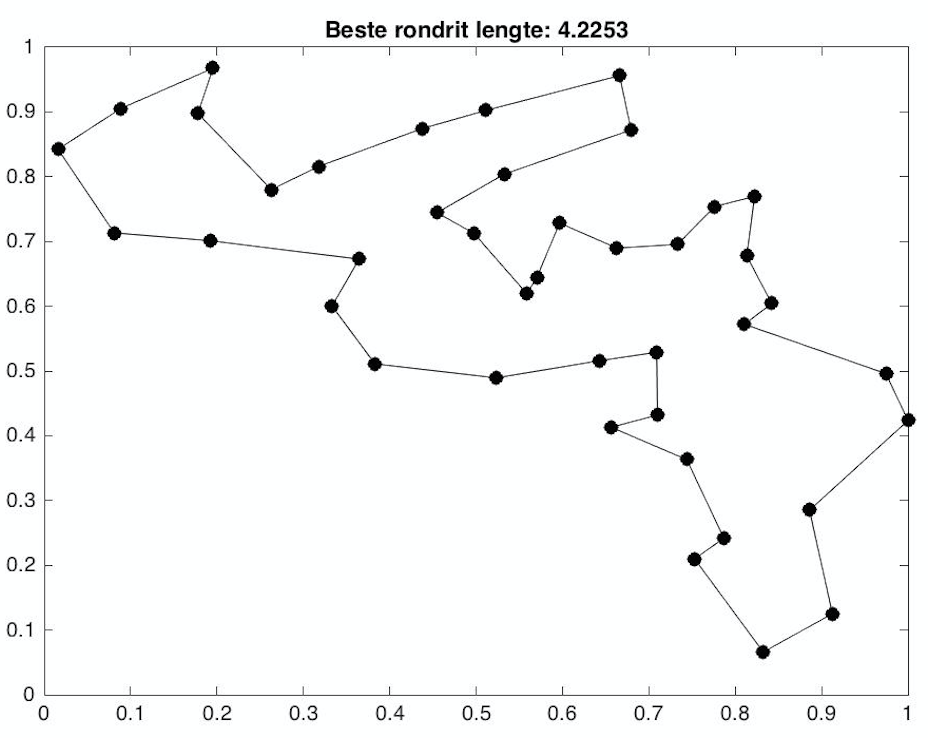
\includegraphics[width=0.5\textwidth]{../figures/figures_question_4/belgium_tour_path}
%      \caption{ There are }
%      \label{fig:belgium_path_4}
%\end{figure}

\begin{figure}[!]
\centering
\begin{subfigure}{.40\textwidth}
  \centering
  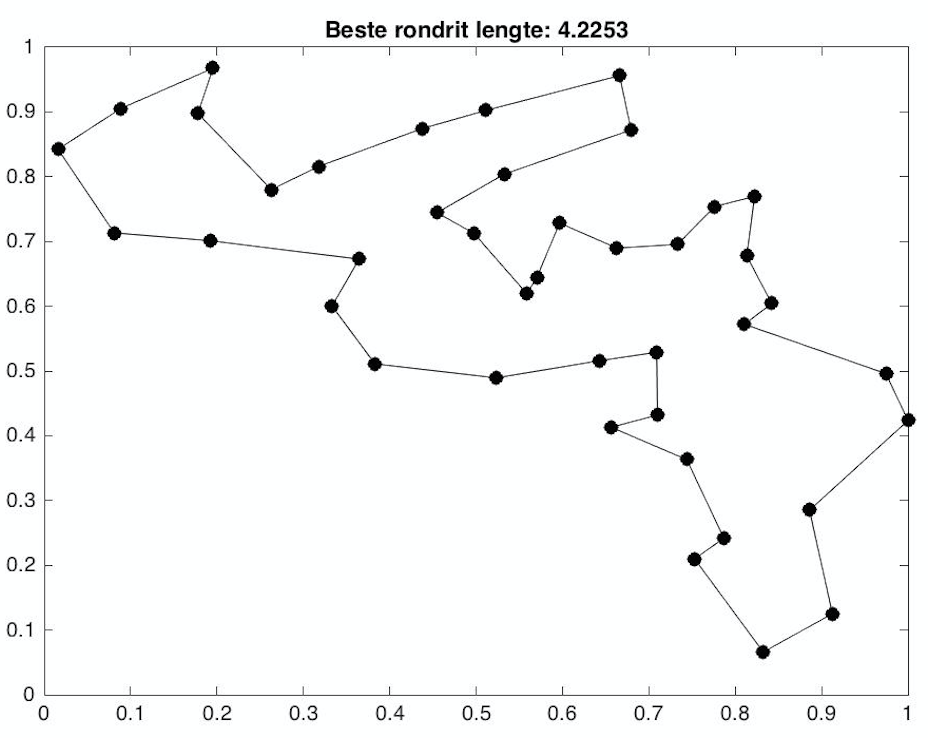
\includegraphics[width=1.2\linewidth]{../figures/figures_question_4/belgium_tour_path}
  \caption{The best tour found for the TSP problem. The distance of the tour is $4.2253$.\\ \ \\}
  \label{fig:belgium_tour_4_path}
\end{subfigure}%
\hspace{0.1\textwidth}
\begin{subfigure}{.45\textwidth}
  \centering
  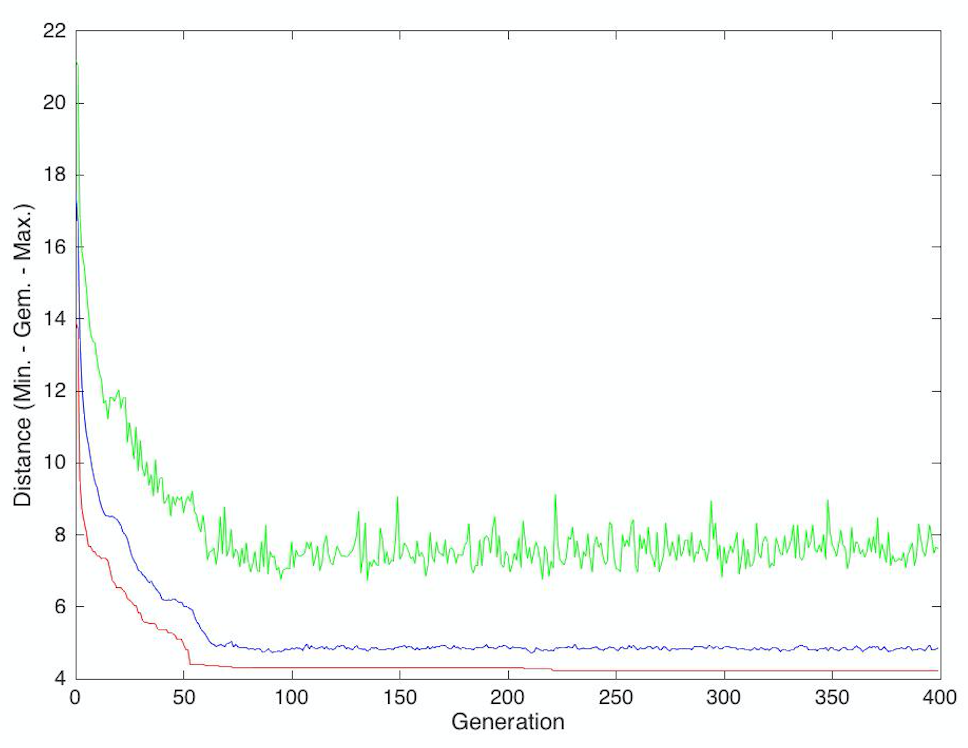
\includegraphics[width=1.2\linewidth]{../figures/figures_question_4/belgium_tour_gen}
  \caption{The fitness values (tour distances) for the best(red), average(blue) and worst(green) candidate solution in every generation. \\}
  \label{fig:belgium_tour_4_gen}
\end{subfigure}
\caption{The benchmark TSP problem \texttt{belgiumtour.tsp} with 41 cities is solved here with path representation, order crossover and inversion mutation. The settings of the GA were \#IND = 400, \#GEN = 400, PR. MUT = $8\%$, PR. CROS = $80\%$, , ELITE = $15\%$, LP DET = ON.}
\label{fig:belgium_tour_4}
\end{figure}

\begin{figure}[!]
\centering
\begin{subfigure}{0.45\textwidth}
  \centering
  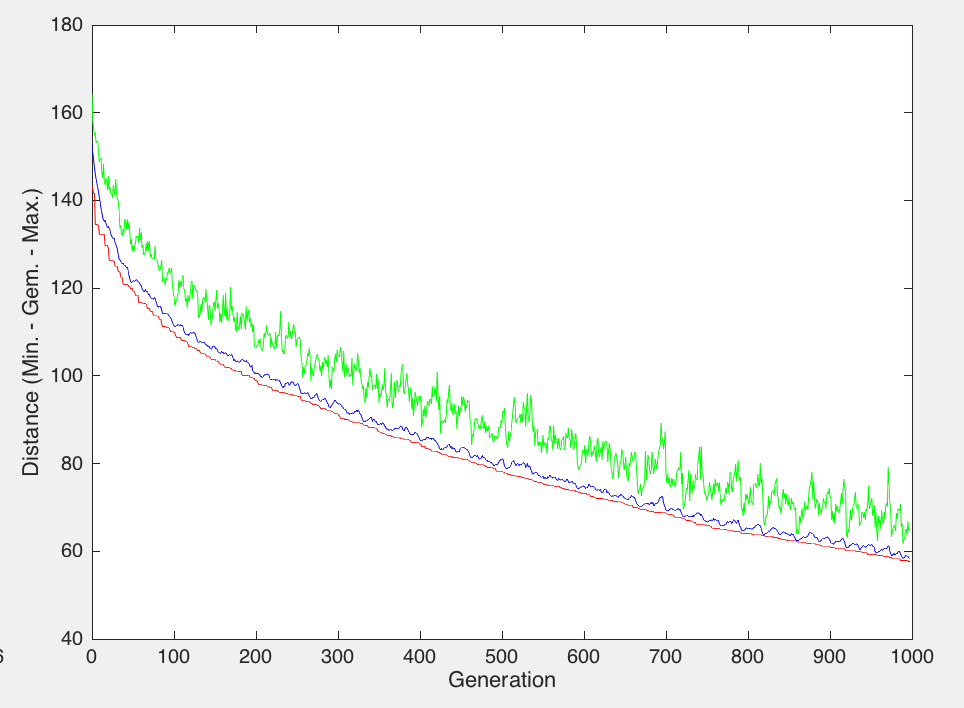
\includegraphics[width=1\textwidth]{../figures/figures_question_4/adj_vraag4_off_gen}
      \caption{\textbf{Adjacency representation (original GA)}. \textbf{Best tour distance found: $\mathbf{57.14}$, computation time: 209 seconds}. PR. MUT = $20\%$, PR. CROS = $50\%$ , ELITE = $10\%$. 200 individuals and 1000 generations.} 
      \label{fig:adj_vraag4_off_gen}
\end{subfigure}%
\hspace{0.05\textwidth}
\begin{subfigure}{0.45\textwidth}
  \centering
  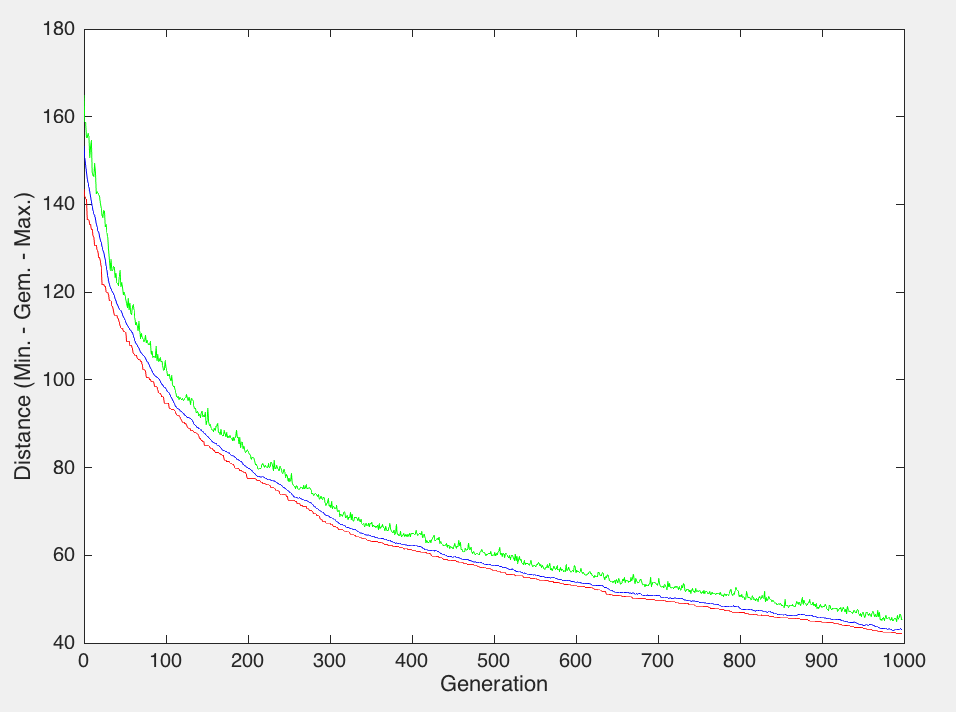
\includegraphics[width=1\textwidth]{../figures/figures_question_4/path_vraag4_off_gen}
      \caption{\textbf{Path representation (new designed GA)}.  \textbf{Best tour distance found: $\mathbf{42.1}$, computation time:357 seconds}.PR. MUT = $8\%$, PR. CROS = $80\%$ , ELITE = $15\%$. 200 individuals and 1000 generations} 
      \label{fig:path_vraag4_off_gen}
\end{subfigure}
\caption{The benchmark TSP problem \texttt{bcl380.tsp} with 380 cities is solved here with both the template program and the new representation, loop detection is switched off for both.}
\label{fig:tour380_off}
\end{figure}
%%%%%%%%%%%%%%%%%%%%%%%%%%%%%%%%%%%%%%
\begin{figure}[!]
\centering
\begin{subfigure}{0.45\textwidth}
  \centering
    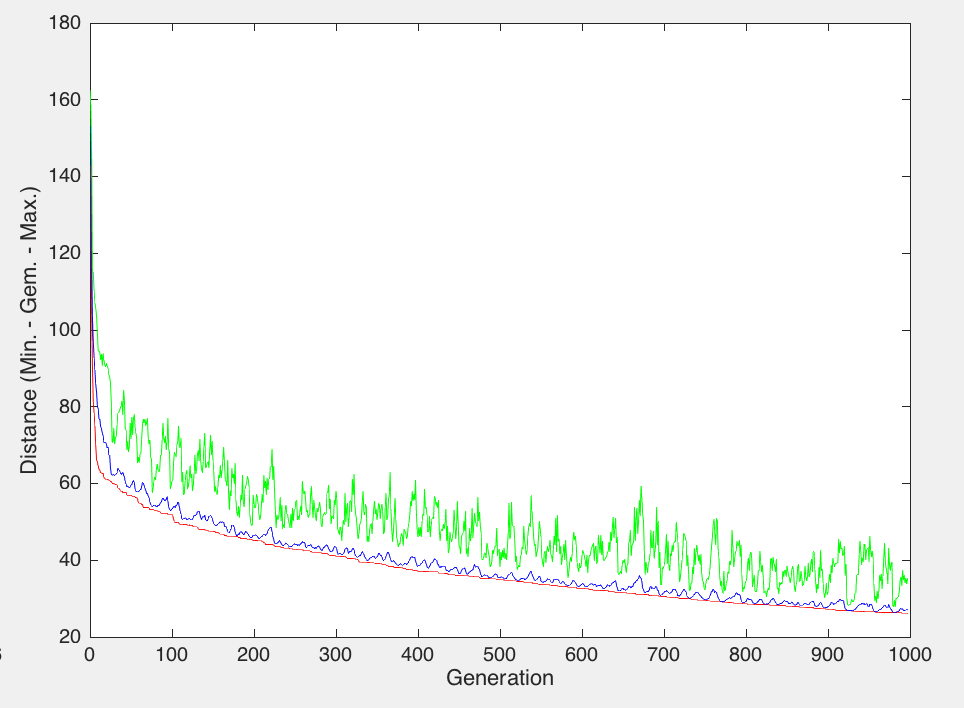
\includegraphics[width=1\textwidth]{../figures/figures_question_4/adj_vraag4_on_gen}
      \caption{\textbf{Adjacency representation (original GA)}. \textbf{Best tour distance found: $\mathbf{26.2}$,computation time:226 seconds}.PR. MUT = $20\%$, PR. CROS = $50\%$ , ELITE = $10\%$. 200 individuals and 1000 generations.}
      \label{fig:adj_vraag4_on_gen}
\end{subfigure}%
\hspace{0.05\textwidth}
\begin{subfigure}{0.45\textwidth}
  \centering
    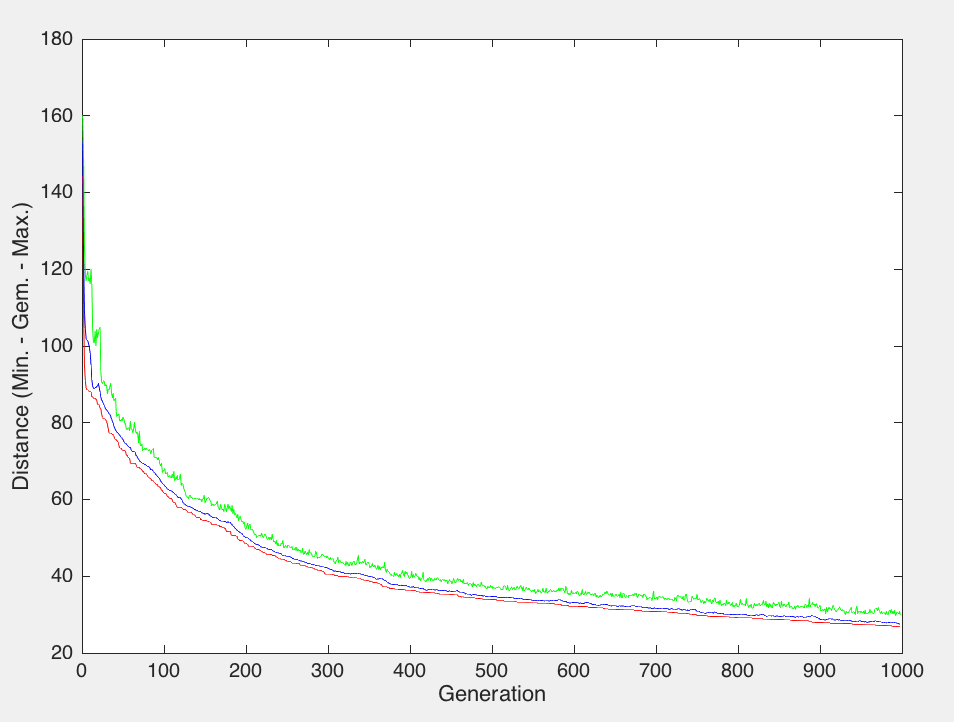
\includegraphics[width=1\textwidth]{../figures/figures_question_4/path_vraag4_on_gen}
      \caption{\textbf{Path representation (new designed GA)}. \textbf{Best tour distance found:  $\mathbf{26.8}$,computation time: 387 seconds}. PR. MUT = $8\%$, PR. CROS = $80\%$ , ELITE = $15\%$. 200 individuals and 1000 generations are used.}
      \label{fig:path_vraag4_on_gen}
\end{subfigure}
\caption{The benchmark TSP problem \texttt{bcl380.tsp} with 380 cities is solved here with both the template program and the new representation, loop detection is switched on for both.}
\label{fig:tour380_on}
\end{figure}















%\begin{figure}[!]
%  \centering
%    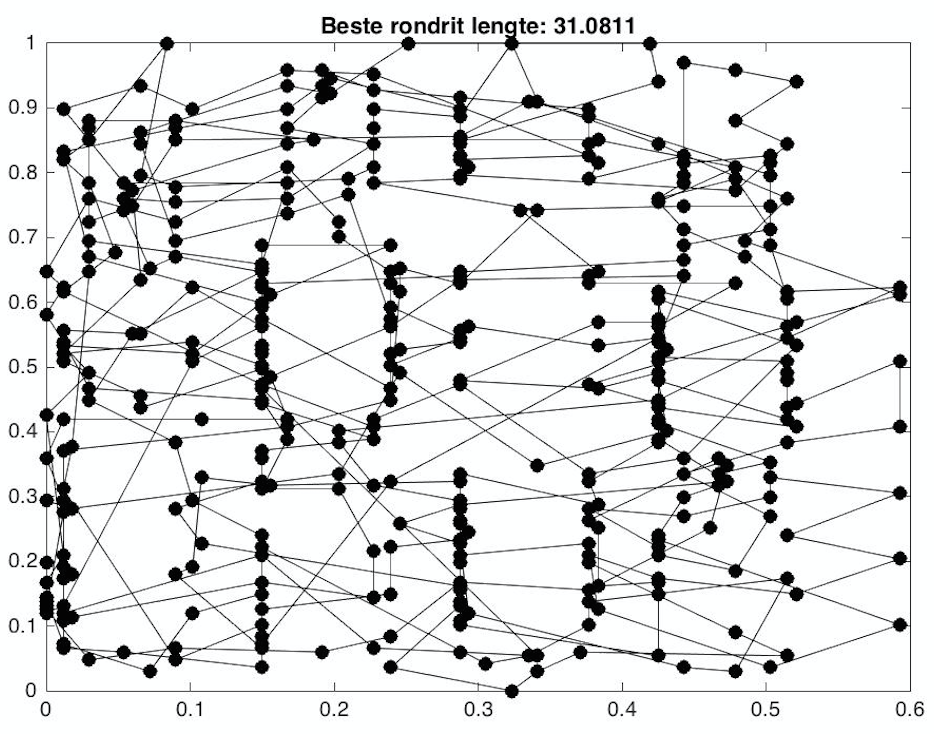
\includegraphics[width=0.7\textwidth]{../figures/figures_question_4/cities380_4_path}
%      \caption{The benchmark TSP problem \texttt{belgiumtour.tsp} with 380 cities is solved here with path representation, order crossover and inversion mutation. The optimal candidate solution is far away from the best solution. The settings of the GA were \#IND = 500, \#GEN = 500, PR. MUT = $8\%$, PR. CROS = $80\%$ , ELITE = $15\%$, LP DET = ON. The CPU time needed was 440 seconds.}
%      \label{fig:cities380_4_path}
%\end{figure}
%
%\begin{figure}[!]
%  \centering
%    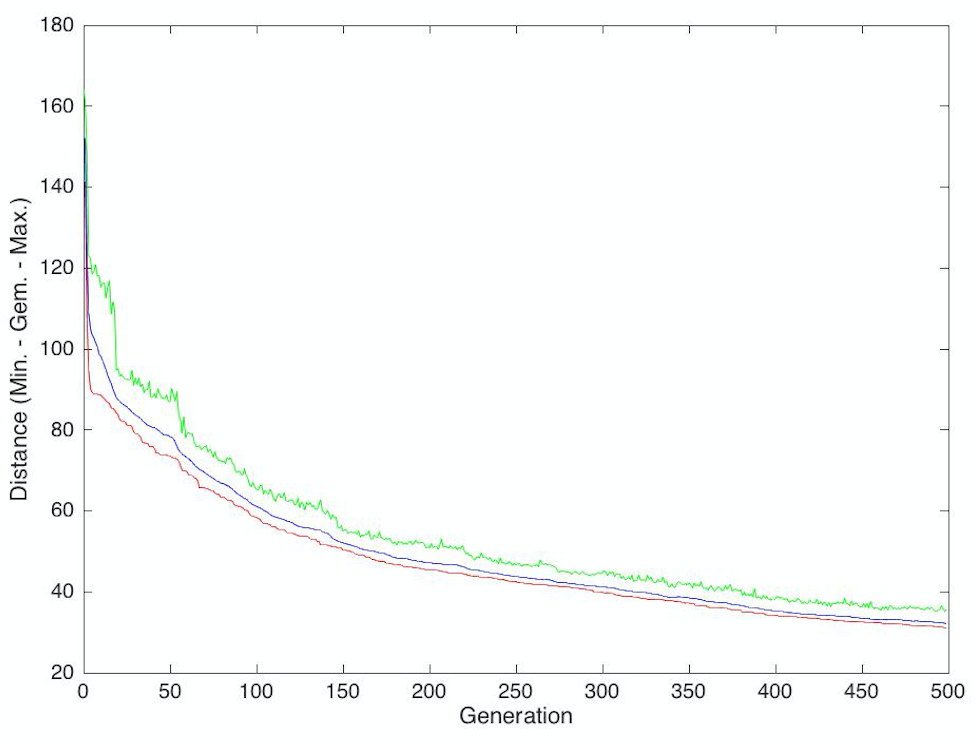
\includegraphics[width=0.7\textwidth]{../figures/figures_question_4/cities380_4_gen}
%      \caption{The fitness values (tour distances) for the best(red), average(blue) and worst(green) candidate solution in every generation. This figure corresponds to the problem solved in figure \ref{fig:cities380_4_path}}
%      \label{fig:cities380_4_gen}
%\end{figure}
%
%\begin{figure}[!]
%  \centering
%    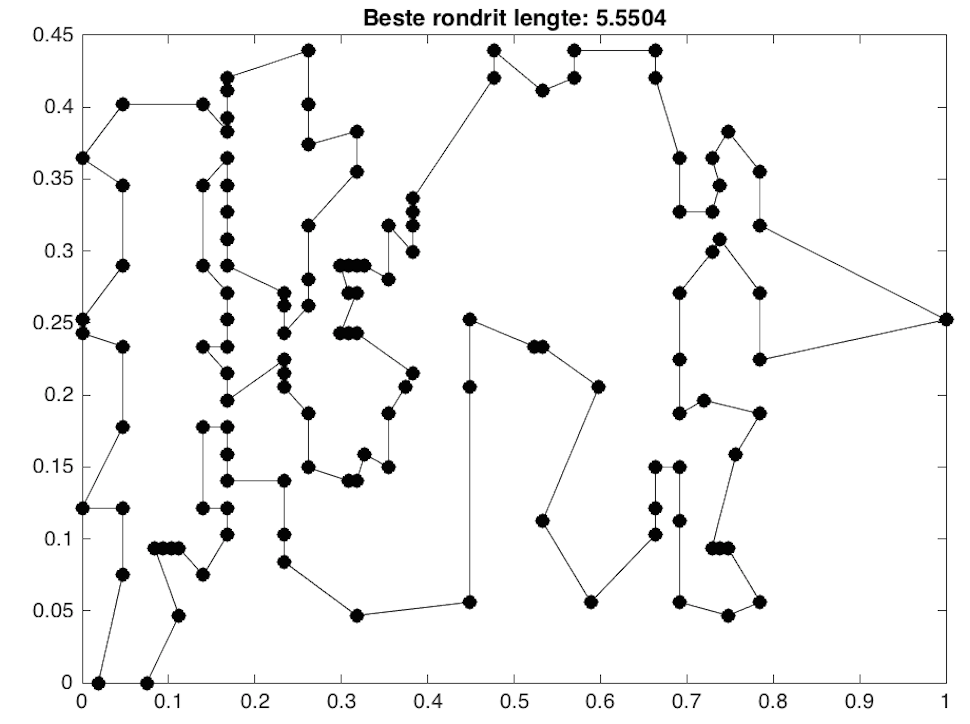
\includegraphics[width=0.7\textwidth]{../figures/figures_question_4/benchmark_131_path}
%      \caption{The benchmark TSP problem \texttt{xqf131.tsp} with 131 cities is solved here with path representation, order crossover and inversion mutation. The optimal candidate solution is very good. The settings of the GA were \#IND = 1000, \#GEN = 1000, PR. MUT = $8\%$, PR. CROS = $80\%$ , ELITE = $15\%$, LP DET = ON. The CPU time needed was 584 seconds.}
%      \label{fig:benchmark_131_path}
%\end{figure}
%
%\begin{figure}[!]
%  \centering
%    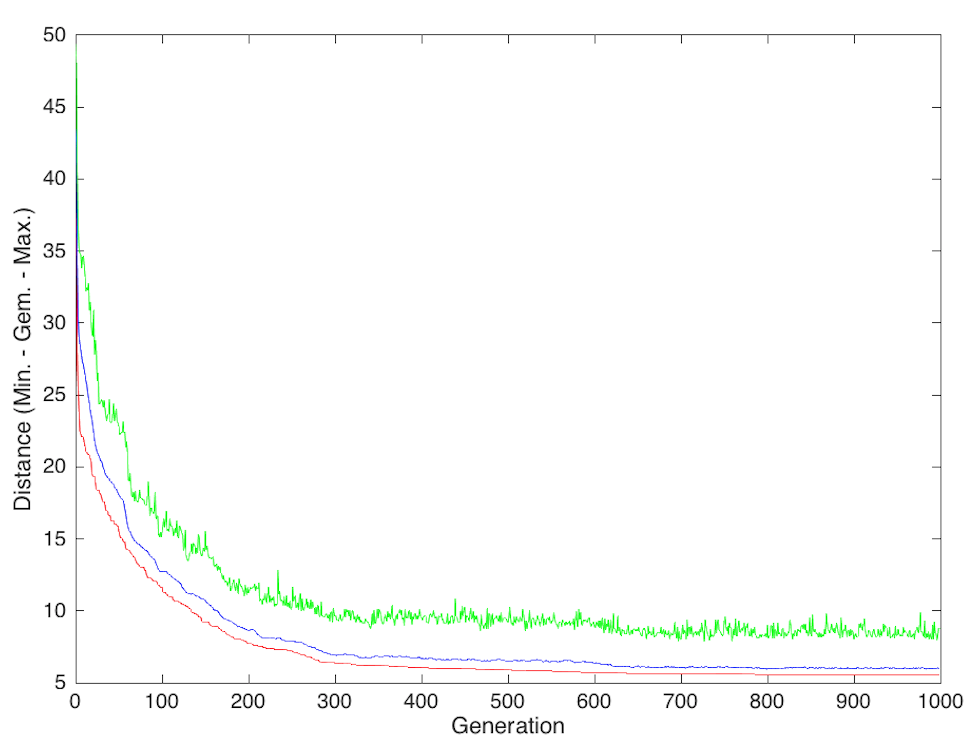
\includegraphics[width=0.7\textwidth]{../figures/figures_question_4/benchmark_131_gen}
%      \caption{The fitness values (tour distances) for the best(red), average(blue) and worst(green) candidate solution in every generation. This figure corresponds to the problem solved in figure \ref{fig:benchmark_131_path}}
%      \label{fig:benchmark_131_gen}
%\end{figure}



\FloatBarrier